\documentclass{article}


\usepackage{array}
\usepackage{float}
\usepackage{makecell}
\usepackage{pgfplots}
\usepackage{amsmath}
\usepackage{amsfonts}
\usepackage{hyperref}

\author{Chirvasa Matei \& Rotariu George}
\title{A study on the application of the Hill Climbing algorithm}

\begin{document}
\maketitle

\section {Abstract}
In this article we will observe the behaviour of the Hill Climbing\cite{HC} algorithm through the perspective of the selection neighbourhood. By considering the neighbourhood of a point to be the set of points that are at Hamming Distance\cite{HD} 1 from the selected point we admit unexpected local maxima to the given function.

\section {Introduction}
We will be studying a commonly used heuristic method, namely Hill Climbing. The two improvement methods used to observe the behaviour of the algorithm are Best Improvement and First Improvement. The Best Improvement or Steepest Ascent selection method works by looking at every neighbour of the selected point and picking the one which is closest to the solution we want. On the other hand, the First Improvement selection method works by iterating through the neighbours of the selected point and picking the first point that is a better solution than the selected one.
\subsection{Motivation}
By observing the effect of the encoding of data on specific instances of a problem we better our understanding of the algorithm altogether. The best way to grasp the effect of the Hill Climbing algorithm, or any algortihm for that matter, is to follow the steps it takes in solving a problem and study and interpret the results it provides.


\section {Method}
\subsection{Function}
The study of the heuristic algorithm will be conducted on the following polynomial function:
$$f(x) = x^3 - 60 \cdot x^2 + 900 \cdot x + 100,
x \in \left[ 0, 31 \right]$$
We will only consider the one dimensional form of the function, plotted in the graph below.\\

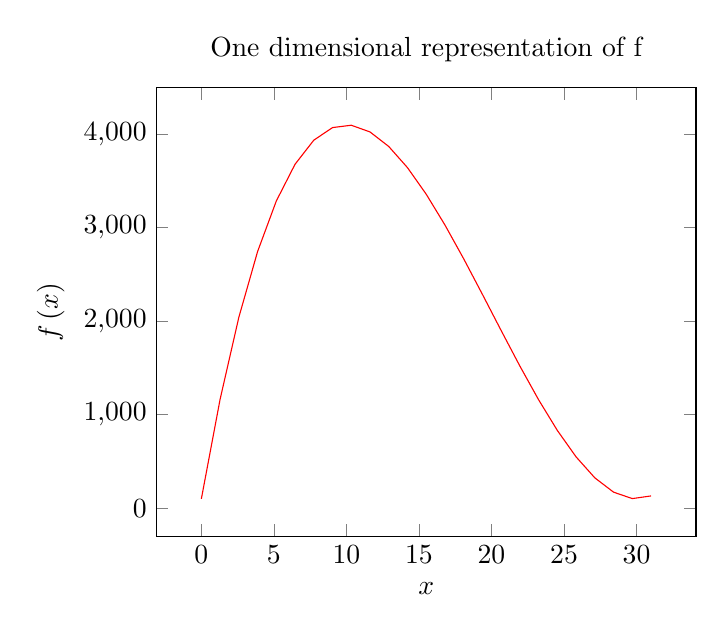
\begin{tikzpicture}
    \begin{axis}[
        title = One dimensional representation of f,
        xlabel={$x$},
        ylabel={$f\left(x\right)$}
    ]
    \addplot[domain=0:31, color=red]{x^3 - 60 * x^2 + 900 * x + 100};
    \end{axis}
\end{tikzpicture}

\subsection{Algorithms}
In this version of the Hill Climbing algorithm we will interpret any point inside the function domain $$\left[0, 31 \right]$$ to be a string of 5 bits representing the base 2 form of every natural number inside the domain. As such, we will consider the neighbourhood $N$ of a point $x_0$  to be the set of bit 5 bit strings that are at Hamming Distance 1 away from $x_0$. More formally, 
$$ \text{N}\left(x_0\right) = \left\{x | x \in \left\{0, 1\right\}^5, \text{HD}(x, x_0) = 1\right\}$$
where
$$\text{HD}:\left\{0, 1\right\}^5 \times \left\{0, 1\right\}^5 \to \mathbb{N}$$
 is the Hamming distance function.
The transformation of data from real values to binary strings combined with the new definition of a neighbourhood of a point leads to a different interpretation of local maxima. 


\section {Experiment}
For the experiment we will calculate the attraction pool of every local maxima in the search domain. The attraction pool $P$ of a local maximum point $x_m$ consists of the points from which if we start to Hill Climb we arrive at $x_m$. The Best Improvement and First Improvement selection methods should generate different attraction pools for the local maxima, however the local maxima found by the two must be the same. This is true due to the fact that both Best and First Improvement declare a point to be local maximum when it proves to be a better solution than its entire neighbourhood. Also, the set of $P$ across all $x_m$ local maxima of $f$ must be a partition of the search domain. This is true due to the fact that from each point in the search domain we arrive at a local maximum after we Hill Climb, so it has to be part of at least one attraction pool and each point has its unique path it takes to arrive there, so it cannot be part of different attraction pools.

\section {Results}

    \begin{figure}[H]
        \centering
        \begin{tabular}{|>{\centering}m{1.5cm}|>{\centering}m{1cm}|>{\centering\arraybackslash}m{8cm}|}
            \hline
            Local maxima & f($x$) & Attraction pool \\
            \hline
            \hline
            01100 & 3988 & $\makecell{00100,\ 01100,\ 11100}$ \\
            \hline
            00111 & 3803 & $\makecell{00110,\ 00111,\ 10110,\ 10111}$ \\
            \hline
            01010 & 4100 & $\makecell{00000,\ 00001,\ 00010,\ 00011,\ 00101,\ 01000,\ 01001,\\ 01010,\ 01011,\ 01101,\ 01110,\ 01111,\ 10101,\ 11000, \\11001,\ 11010,\ 11011,\ 11101,\ 11110,\ 11111}$ \\
            \hline
            10000 & 3236 & $\makecell{10000,\ 10001,\ 10010,\ 10011,\ 10100}$ \\
            \hline
        \end{tabular}
        \caption{Attraction pools of local maxima using the Best Improvement selection method}
    \end{figure}


    \begin{figure}[H]
        \centering
        \begin{tabular}{|>{\centering}m{1.5cm}|>{\centering}m{1cm}|>{\centering\arraybackslash}m{8cm}|}
            \hline
            Local maxima & f($x$) & Attraction pool \\
            \hline
            \hline
            01100 & 3988 & $\makecell{00100,\ 01000,\ 01100,\ 10100,\ 11000,\ 11100}$ \\
            \hline
            00111 & 3803 & $\makecell{00111,\ 01111,\ 10111,\ 11111}$ \\
            \hline
            01010 & 4100 & $\makecell{00101,\ 00110,\ 01001,\ 01010,\ 01011,\ 01101,\ 01110,\\ 10101,\ 10110,\ 11001,\ 11010,\ 11011,\ 11101,\ 11110}$ \\
            \hline
            10000 & 3236 & $\makecell{00000,\ 00001,\ 00010,\ 00011,\ 10000,\ 10001,\ 10010,\\ 10011}$ \\
            \hline
        \end{tabular}
        \caption{Attraction pools of local maxima using the First Improvement selection method}
    \end{figure}

\subsection{Interpretation}
As can be seen, compared to the real interpretation of points and neighbourhoods, the binary interpretation of points and the Hamming neighbourhood not only generate different local maxima, but also created more local maxima than present in the real function representation. We may also notice that, in this specific situation, Best Improvement had a better probability of starting of with a bitstring that would lead to the global maxima of the function.

\section {Conclusions}
Given the experiment's results, we may conclude that our hypothesis regarding the different encoding and representation of neighbouring values depending on encoding was correct, and as such we obtained multiple local maxima in an unimodal function when representing numbers as bits strings, and obtained different neighbouring fields, with 2 neighbours when using real number representation and 5 neighbours, the number of bits, when using a Hamming Distance of 1 as the method of finding them. This shows a possible flaw in encoding, as we failed to always find the global maxima of a unimodal function. However, this could pose an advantage in different scenarios, and this has presented the possibility of mixing both types of encoding to further improve the results of a Hill Climbing algorithm.

\begin{thebibliography}{9}

\bibitem{HC}
``Hill climbing'', Wikipedia, Wikimedia Foundation, 23 March 2023, \url{https://en.wikipedia.org/wiki/Hill\_climbing}

\bibitem{HD}
``Hamming distance'', Wikipedia, Wikimedia Foundation, 23 September 2023, \url{https://en.wikipedia.org/wiki/Hamming\_distance}

\bibitem{GA}
Eugen Nicolae Croitoru, Department of Computer Science ``Alexandru Ioan Cuza'' University of Iasi, Romania, ``Teaching: Genetic Algorithms'', retrieved October 31, 2023, from \url{https://profs.info.uaic.ro/~eugennc/teaching/ga/}

\end{thebibliography}

\end{document}